\documentclass[UTF8,12pt,a4paper]{ctexart}

\usepackage{amsmath}
\usepackage{cases}
\usepackage{cite}
\usepackage{graphicx}
\usepackage{enumerate}
\usepackage{algorithm}
\usepackage{caption}   % \caption*需要
\usepackage{subcaption} % 子图布局
\usepackage[noend]{algpseudocode} %algorithmicx
\makeatletter
\renewcommand{\fnum@algorithm}{\fname@algorithm}
\makeatother
\renewcommand{\algorithmicrequire}{\textbf{Input:}}
\renewcommand{\algorithmicensure}{\textbf{Output:}}
\usepackage[margin=1in]{geometry}
\geometry{a4paper}
\usepackage{fancyhdr}
\pagestyle{fancy}
\fancyhf{}
\usepackage{xcolor}

% ------------------- 健全表格环境 ----------------------
\usepackage{tabularx}
\usepackage{booktabs} % 三线表
\usepackage{multirow}
% ------------------- 自定义代码展示风格 -----------------
\usepackage{listings}
\usepackage{xcolor}
\lstdefinestyle{hspice}{
    language=C,
    basicstyle=\ttfamily\small,
    keywordstyle=\color{blue}\bfseries,
    commentstyle=\color{green!50!black},
    stringstyle=\color{brown},
    numbers=left,
    numberstyle=\tiny\color{gray},
    stepnumber=1,
    numbersep=5pt,
    backgroundcolor=\color{white},
    showspaces=false,
    showstringspaces=false,
    showtabs=false,
    frame=single,
    rulecolor=\color{black},
    tabsize=2,
    captionpos=b,
    breaklines=true,
    breakatwhitespace=true,
    escapeinside={\%*}{*)},
    morekeywords={param, include, temp, option, probe, DC, dc, measure, alter, VDD, GND, gnd, NMOS, PMOS,FIND, WHEN, sweep, abs, I, SUPPLY, lg, fin_height, fin_width, tran, ac, op, model, end, subckt,ends,global, nmos, pmos, inv, data, +}, % 根据需要添加更多HSPICE关键字
    comment=[l]{*} % 在这里设置注释
}

\lstset{style=hspice} % 只应用样式



% ------------------- 设置超链接，便于跳转 -----------------
\usepackage{enumitem}
\usepackage{hyperref}
\hypersetup{
    pdfborder={0 0 0},    % 消除超链接边框
    colorlinks=true,       % 将边框改为颜色标记（可选）
    linkcolor=black,       % 内部链接颜色（目录、引用等）
    citecolor=black,       % 引用颜色
    urlcolor=blue          % URL链接颜色（保持蓝色以便区分）
}




% ------------------------ 标题区 ----------------------------
\title{DIC Lab3 Report}
\author{
	姓名：\underline{冯峻}~~~~~~
	学号：\underline{523031910148}~~~~~~}
\date{\today}
\pagenumbering{arabic}

\begin{document}



% ------------------------ 页眉和页脚 ----------------------------
\fancyhead[L]{冯峻}
\fancyhead[C]{Lab3 Report}
\fancyfoot[C]{\thepage}

\maketitle
%\tableofcontents
%\newpage

%================================================================================
% Introduction and background
%================================================================================
\section{Introduction and background}
本项目基于逻辑努力（Logical Effort）方法对数字电路进行优化，旨在通过合理选择电路中各个逻辑门的尺寸，以最小化信号传播延迟。逻辑努力是一种通过分析电路中每个逻辑门的延迟和负载来指导电路设计的方法。

然而，理论与实际有不可避免的偏差，但是基于逻辑努力的分析方法依旧可以为我们指明一个方向。我们可以根据这一方法分析电路中各个逻辑门、晶体管的尺寸参数范围，在此基础上，借助仿真工具，通过对电路进行建模和仿真，我们可以找到最佳的门尺寸组合，从而提高电路性能。

\subsection{实验全局配置}
本实验采用HSPICE进行电路仿真，仿真环境配置如下：

\begin{enumerate}
    \item 工艺库：PTM 16HP FinFETs
    \item 仿真等级：RUNLVL = 6
    \item 栅极长度：$L_g = 20$nm
    \item 供电电压：$V_{\text{DD}} = 0.75$V
    \item 仿真温度：$T = 25^\circ\mathrm{C}$
\end{enumerate}

\subsection{逻辑门的HSPICE定义}
\textbf{1. Inverter}
\begin{lstlisting}
* Sub circuit: Inverter definition
.subckt INV in out vdd gnd size=1
Mn out in gnd gnd nfet L='Lg' NFIN ='size'
Mp out in vdd vdd pfet L='Lg' NFIN ='size'
.ends INV
\end{lstlisting}

\textbf{2. 2-NAND}
\begin{lstlisting}
* Sub circuit: 2-NAND
.subckt NAND2 in1 in2 out vdd gnd size=1 Lg=20n
* PUN
Mp1 out in1 vdd vdd pfet L='Lg' NFIN='size'
Mp2 out in2 vdd vdd pfet L='Lg' NFIN='size'
* PDN
Mn1 out in1 source1 gnd nfet L='Lg' NFIN='size'
Mn2 source1 in2 gnd gnd nfet L='Lg' NFIN='size'
.ends NAND2
\end{lstlisting}


\textbf{3. 2-NOR}
\begin{lstlisting}
* Sub circuit: 2-NOR
.subckt NOR2 in1 in2 out vdd gnd size=1 Lg=20n
*PUN
Mp1 out in1 source_p1 vdd pfet L='Lg' NFIN='size'
Mp2 source_p1 in2 vdd vdd pfet L='Lg' NFIN='size'
*PDN
Mn1 out in1 gnd gnd nfet L='Lg' NFIN='size'
Mn2 out in2 gnd gnd nfet L='Lg' NFIN='size'
.ends NOR2
\end{lstlisting}

\textbf{4. 3-NAND}
\begin{lstlisting}
* Sub circuit: 3-NAND
.subckt NAND3 in1 in2 in3 out vdd gnd size=1 Lg=20n
* PUN
Mp1 out in1 vdd vdd pfet L='Lg' NFIN='size'
Mp2 out in2 vdd vdd pfet L='Lg' NFIN='size'
Mp3 out in3 vdd vdd pfet L='Lg' NFIN='size'
* PDN
Mn1 out in1 source1 gnd nfet L='Lg' NFIN='size'
Mn2 source1 in2 source2 gnd nfet L='Lg' NFIN='size'
Mn3 source2 in3 gnd gnd nfet L='Lg' NFIN='size'
.ends NAND3
\end{lstlisting}

\textbf{5. 3-NOR}
\begin{lstlisting}
* Sub circuit: 3-NOR
.subckt NOR3 in1 in2 in3 out vdd gnd size=1 Lg=20n
*PUN
Mp1 out in1 source_p1 vdd pfet L='Lg' NFIN='size'
Mp2 source_p1 in2 source_p2 vdd pfet L='Lg' NFIN='size'
Mp3 source_p2 in3 vdd vdd pfet L='Lg' NFIN='size'
*PDN
Mn1 out in1 gnd gnd nfet L='Lg' NFIN='size'
Mn2 out in2 gnd gnd nfet L='Lg' NFIN='size'
Mn3 out in3 gnd gnd nfet L='Lg' NFIN='size'
.ends NOR3
\end{lstlisting}

Inverter, 2-NAND, 2-NOR的示意图分别见图\ref{fig:Inv}、\ref{fig:NAND2}、\ref{fig:NOR2}。
\begin{figure}[htbp]
    \centering
    \begin{subfigure}{0.32\textwidth}
        \centering
        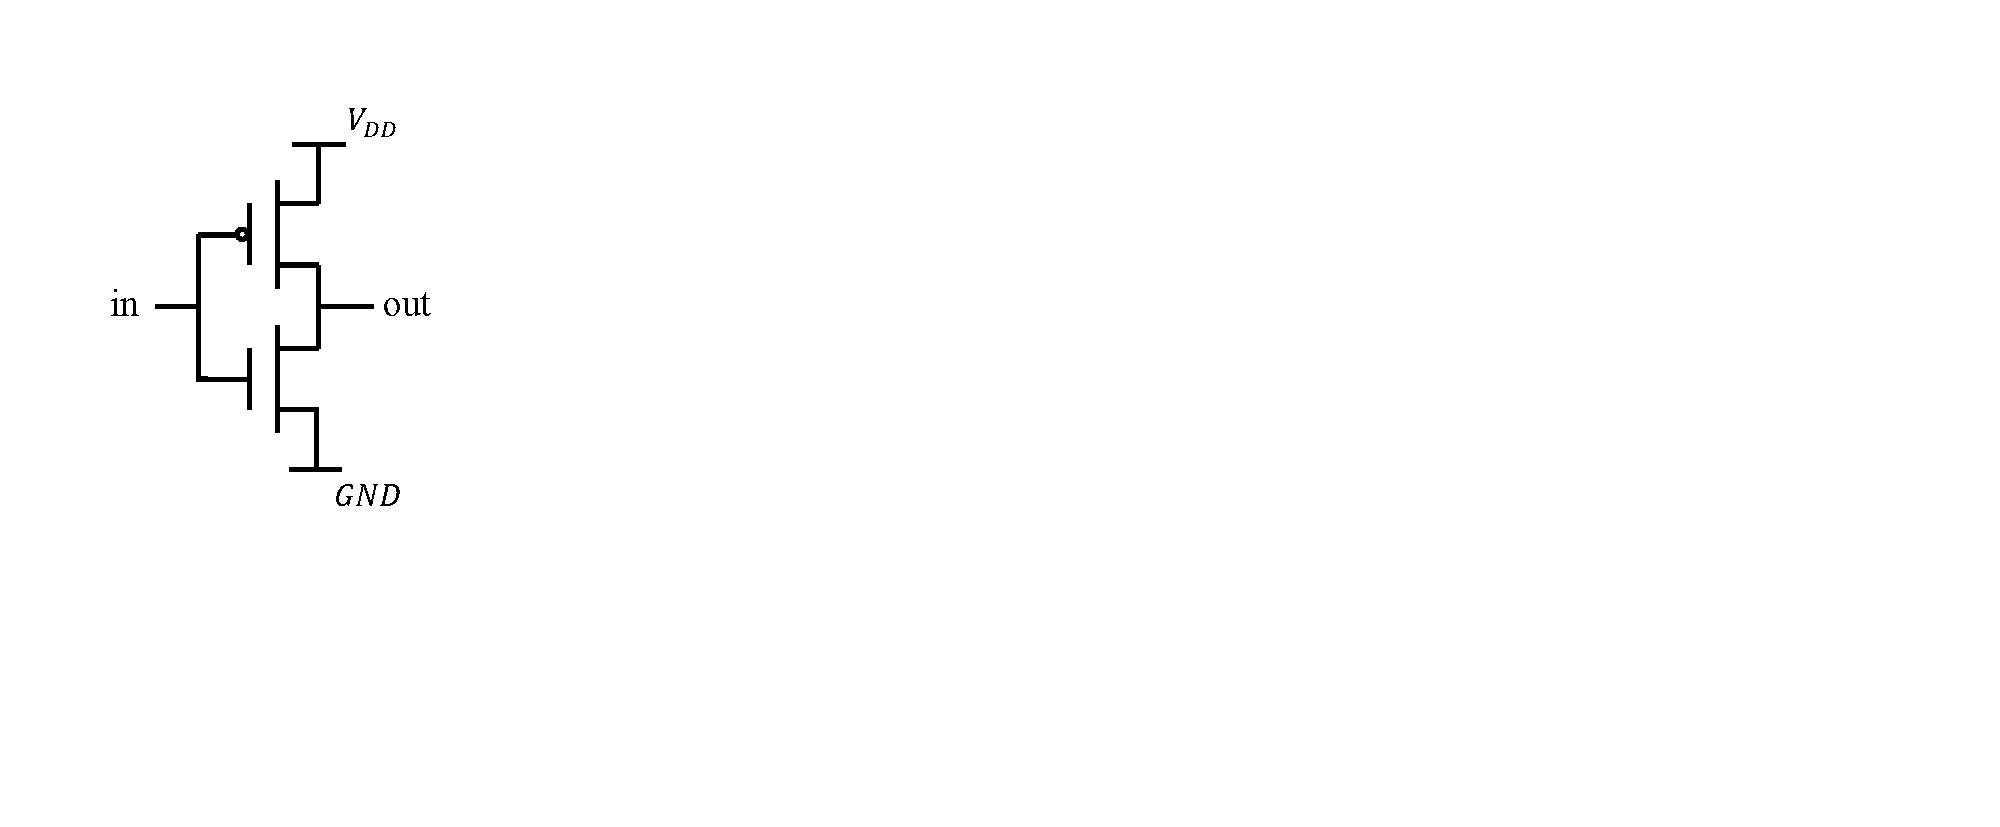
\includegraphics[width=\linewidth]{Inv.pdf}
        \caption{Inverter示意图}
        \label{fig:Inv}
    \end{subfigure}
    \begin{subfigure}{0.32\textwidth}
        \centering
        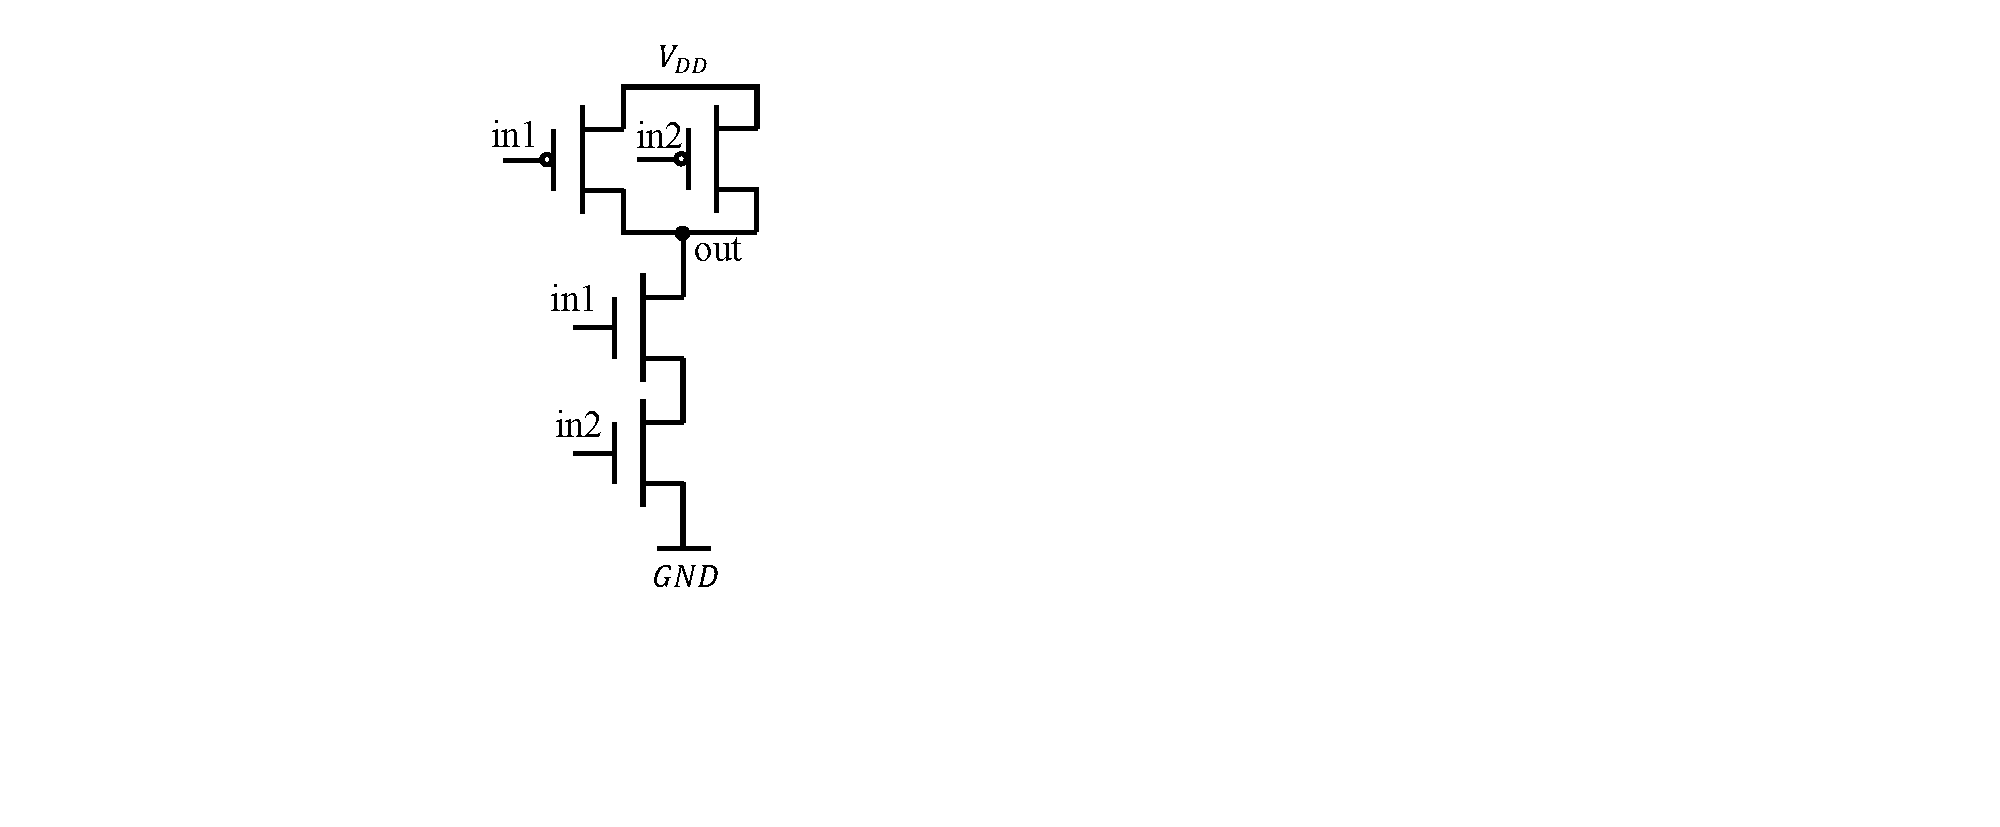
\includegraphics[width=\linewidth]{NAND2.pdf}
        \caption{2-NAND示意图}
        \label{fig:NAND2}
    \end{subfigure}
    \begin{subfigure}{0.32\textwidth}
        \centering
        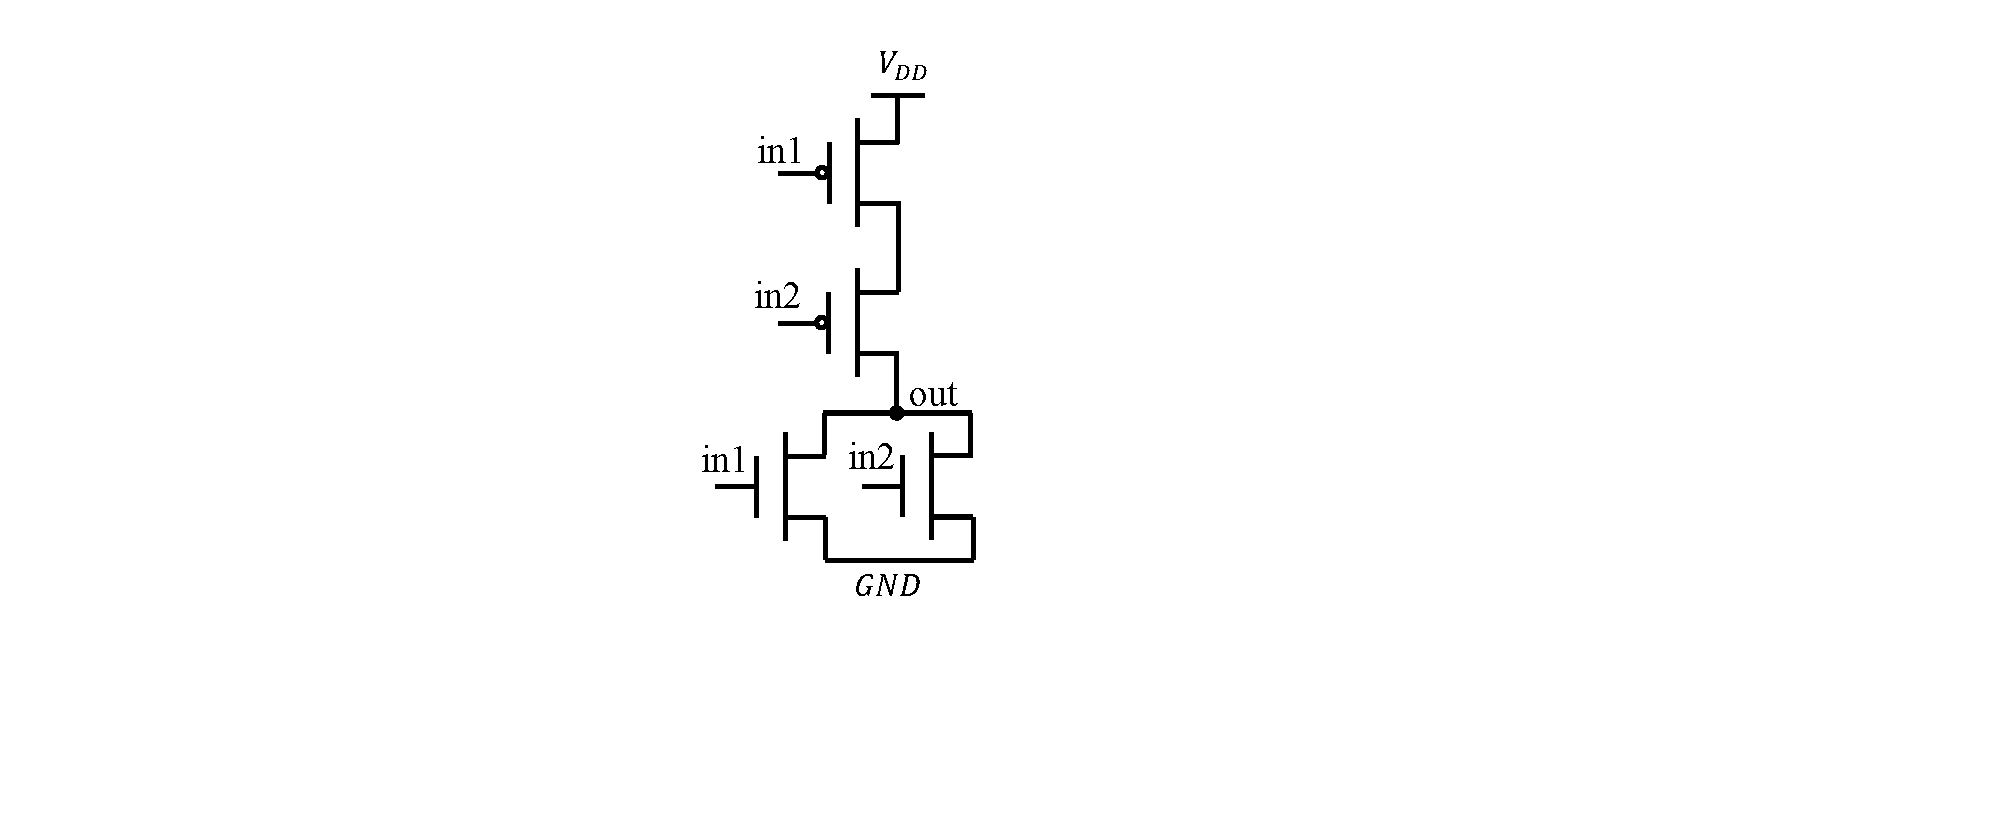
\includegraphics[width=\linewidth]{NOR2.pdf}
        \caption{2-NOR示意图}
        \label{fig:NOR2}
    \end{subfigure}
    \caption{Inverter, 2-NAND, 2-NOR示意图}
\end{figure}

3-NAND, 3-NOR门的示意图分别见图\ref{fig:NAND3}、\ref{fig:NOR3}。
\begin{figure}
    \begin{subfigure}{0.48\textwidth}
        \centering
        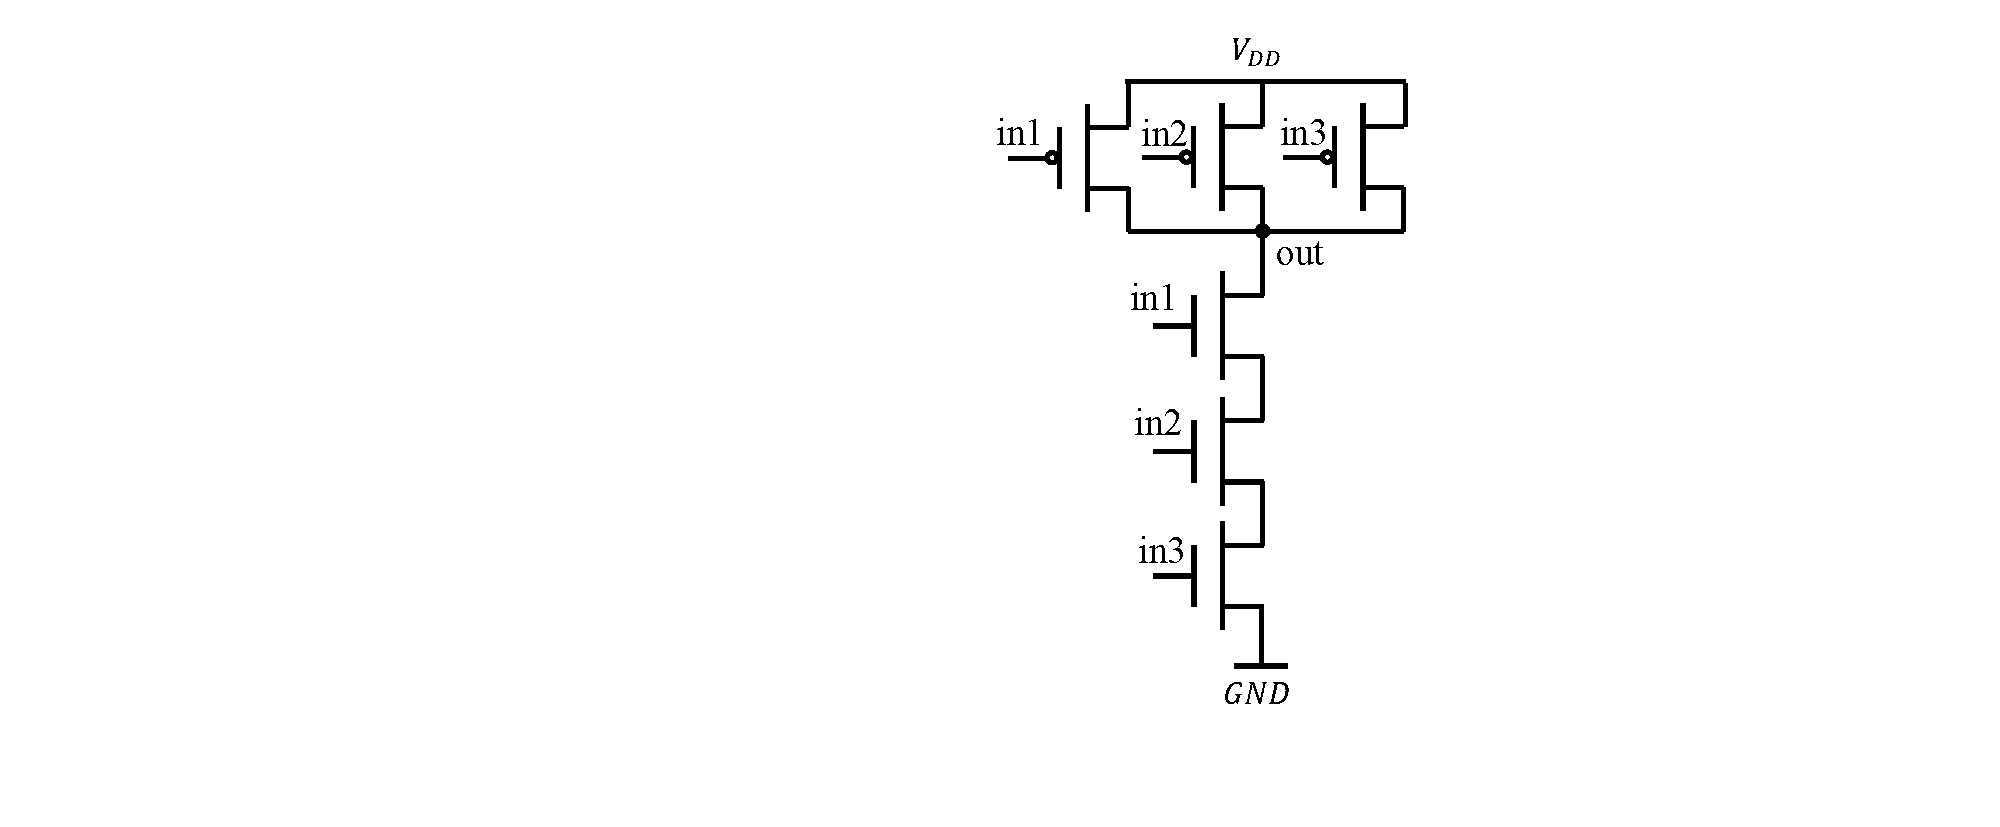
\includegraphics[width=\linewidth]{NAND3.pdf}
        \caption{3-NAND示意图}
        \label{fig:NAND3}
    \end{subfigure}
    \begin{subfigure}{0.48\textwidth}
        \centering
        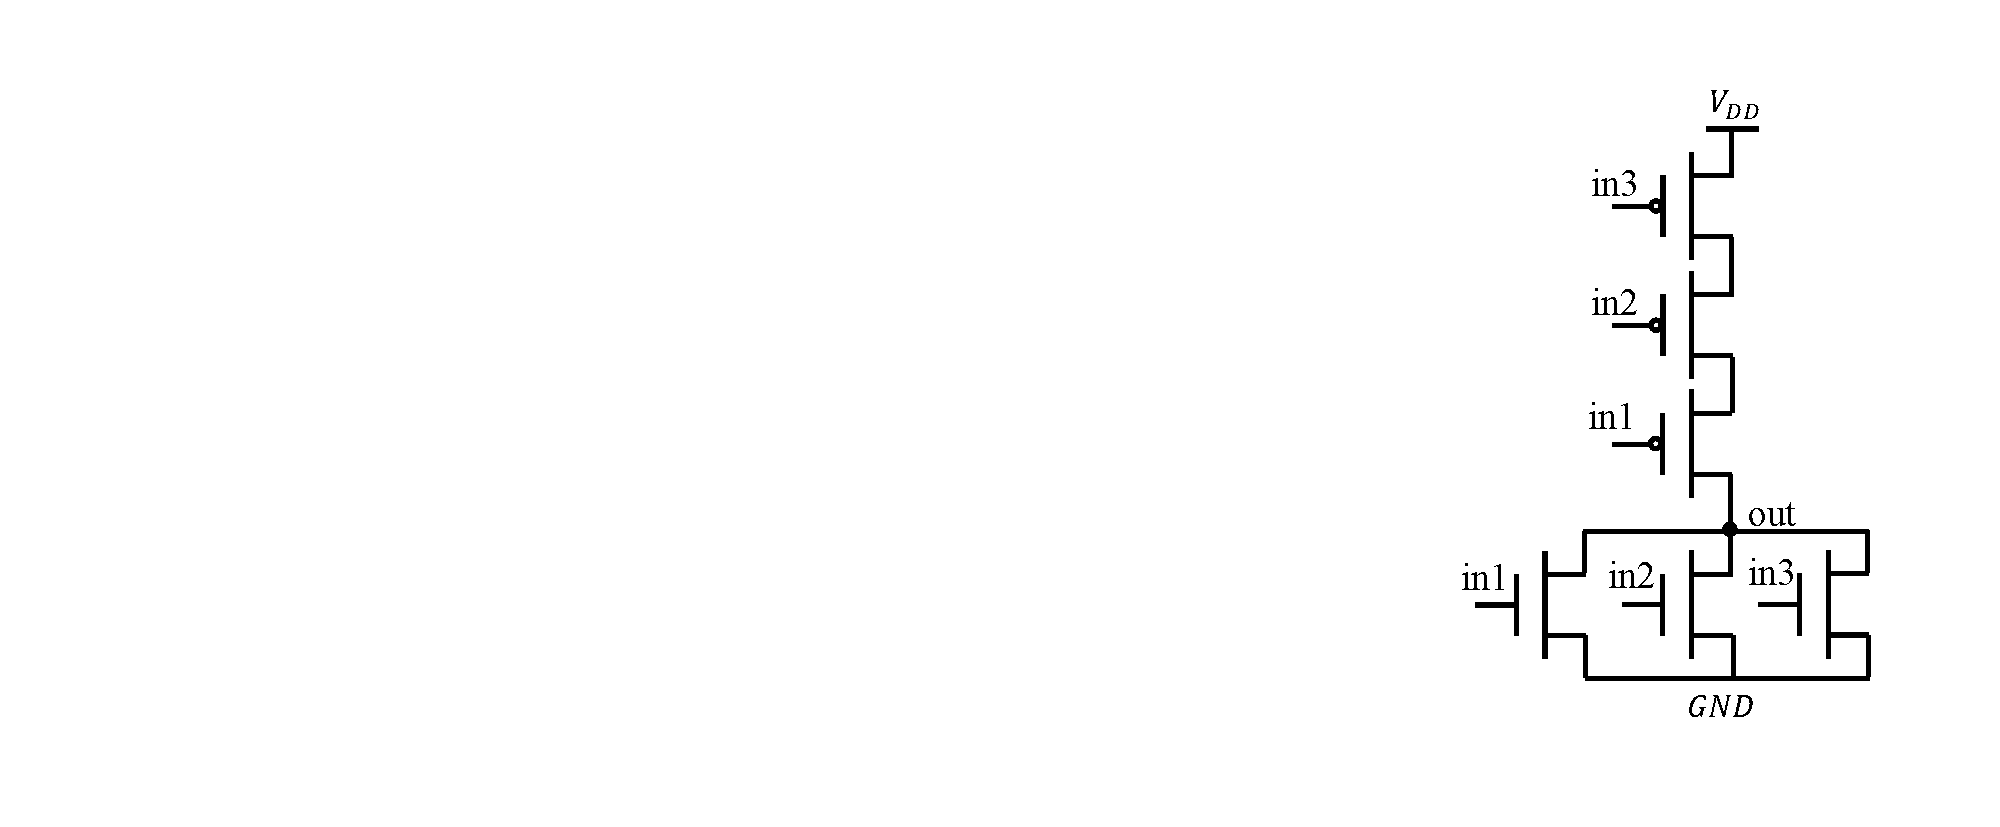
\includegraphics[width=\linewidth]{NOR3.pdf}
        \caption{3-NOR示意图}
        \label{fig:NOR3}
    \end{subfigure}
    \caption{3-NAND, 3-NOR示意图}
\end{figure}

\subsection{仿真说明}
本次SPICE仿真过程中，有几点注意事项：

1. 由于工艺库采用的是16hp FinFET，可以近似认为相同尺寸（$W, L$）的NMOS和PMOS具有相同的电流驱动能力（即具有相同的导通电阻），因此，在构建驱动能力相同的PUN和PDN时，确保PUN和PDN在最坏情况下拥有相同的导通电阻，就是要确保在最坏情况下，PUN和PDN具有相同的等效尺寸。

2. 在1.的前提下，我们利用"NFIN"参数来评判FinFET的尺寸。但是"NFIN"只能是整数，因此，在后续组合逻辑门链优化过程中，计算出来的理论尺寸，实验中采取\textbf{四舍五入}的方式得到实际仿真使用尺寸。

3. 延时的测量方法：测量出在两种输入翻转（从高到低和从低到高）情况下，输出的$t_{\text{pHL}}$和$t_{\text{pLH}}$，然后用\textbf{平均延时}：
$$t_{\text{p}} = \frac{t_{\text{pHL}} + t_{\text{pLH}}}{2}$$
衡量该\textbf{critical path}的性能


%================================================================================
% Task 1: Use Logical Effort to Size Gates
%================================================================================
\newpage
\section{Task 1: Use Logical Effort to Size Gates}
\subsection{实验电路}

本Task研究的组合逻辑门链见图\ref{fig:task1_ckt}
\begin{figure}[htbp]
    \centering
    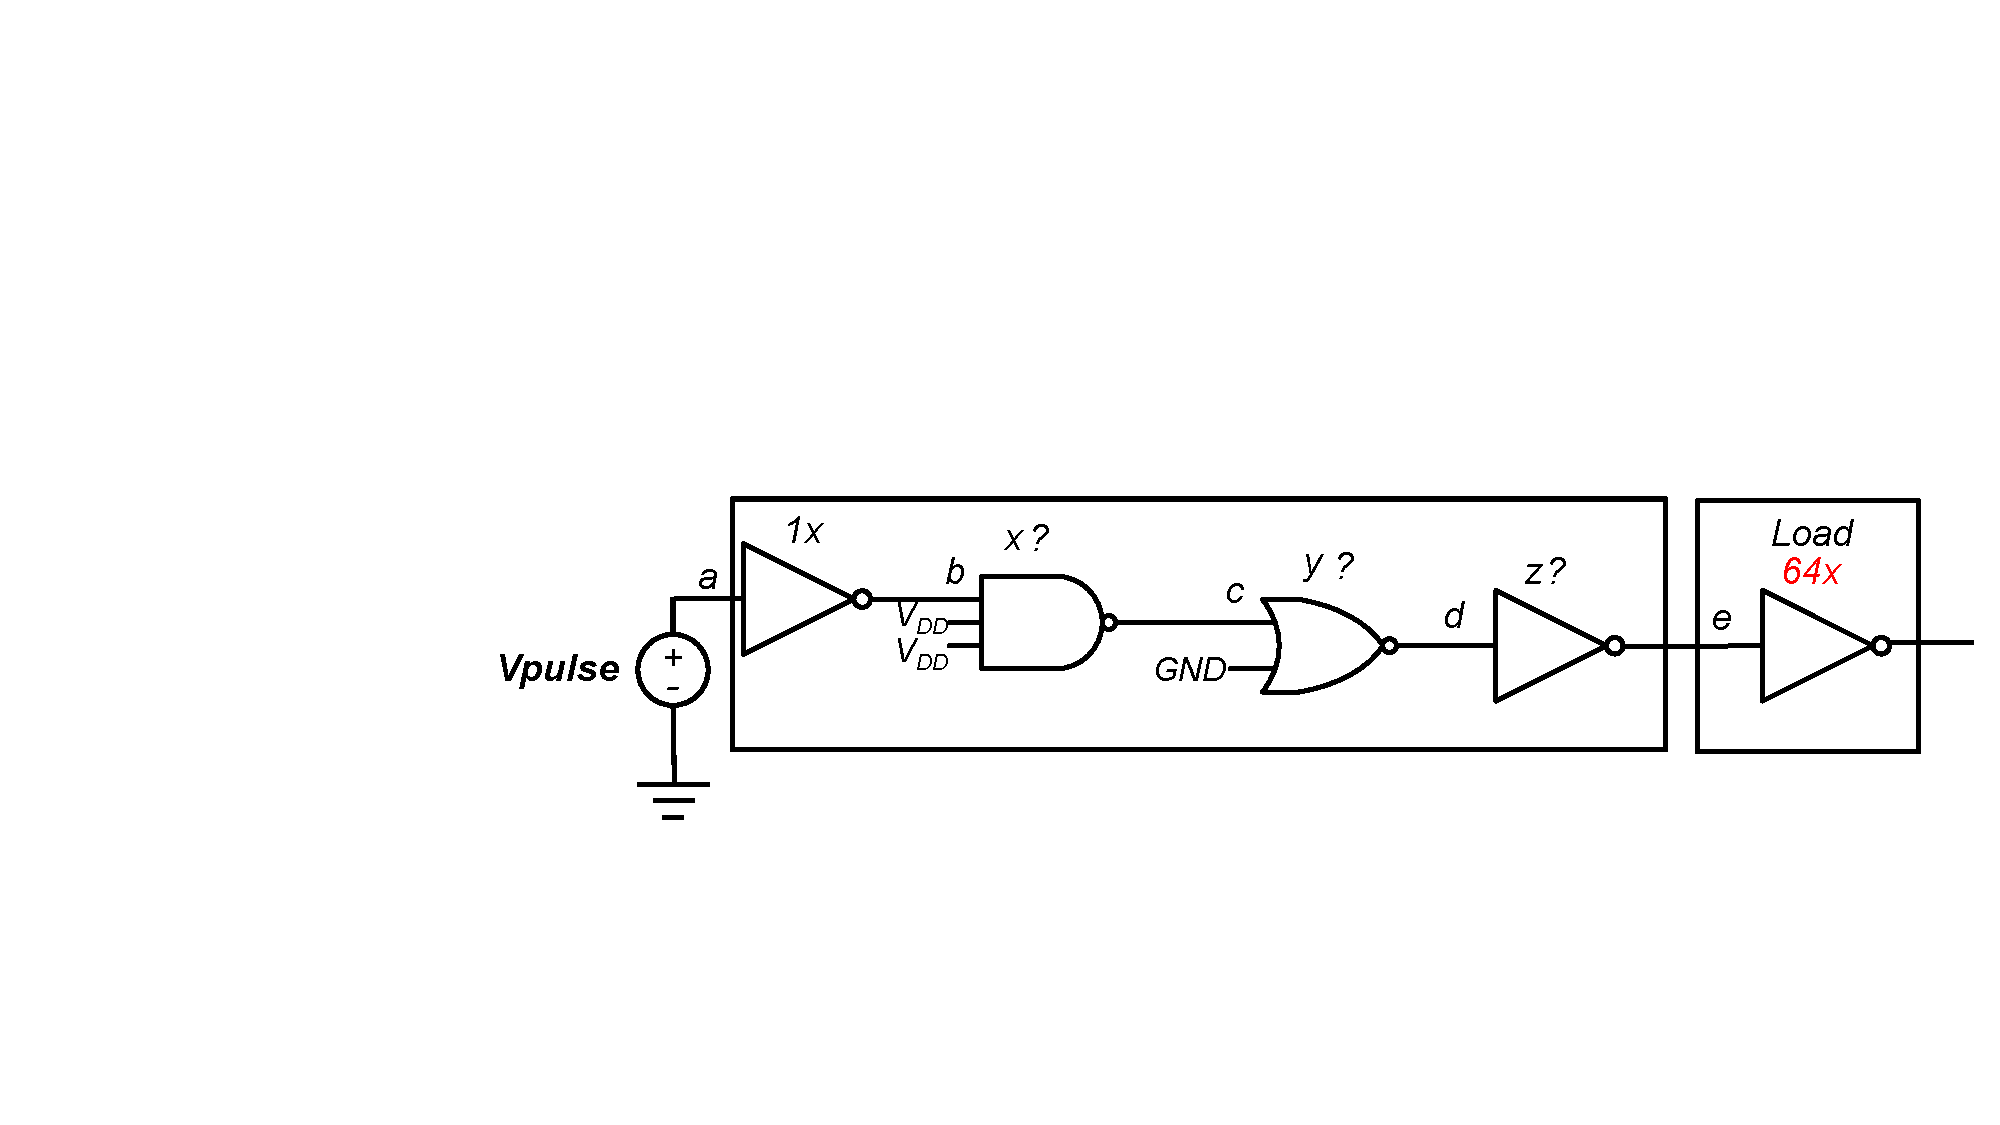
\includegraphics[width=0.8\textwidth]{Task1_ckt.pdf}
    \caption{Task1 电路}
    \label{fig:task1_ckt}
\end{figure}

从图\ref{fig:task1_ckt}可知，电路信号链为：
$$a \rightarrow \text{inv(minimum size)} \rightarrow b \rightarrow \text{3-NAND} \rightarrow c \rightarrow \text{2-NOR} \rightarrow d \rightarrow \text{inv2} \rightarrow e \rightarrow \text{load}(64 \times \text{inv})$$。
其中a作为input, e作为output。

我们需要选择合适的3-NAND、2-NOR、inv2尺寸，以使得从a到e的延迟最小。衡量延时的方法为：$t_p = (t_{pHL} + t_{pLH})/2$。

\subsection{理论优化分析}

\subsubsection{优化方法建模}

我们从已知组合逻辑门能够获取的指标（本征延迟$p$、逻辑努力$g$、尺寸$s$、等效扇出$f$、分支努力$b$）参见表\ref{tab:task1_metrics}（设第一个inv(minimum size)，3-NAND，2-NOR，inv2的参数下标分别为1, 2, 3, 4）

\begin{table}[htbp]
    \centering
    \caption{Task1组合逻辑门链的逻辑门关键指标}
    \label{tab:task1_metrics}
    % 修正：原代码为6列，实际数据只有5列，改为ccccc
    \begin{tabular}{ccccc}
    \toprule
    stage & inv(minimum size) & 3-NAND & 2-NOR & inv2 \\
    \midrule
    $p$ & $p_1 = 1$ & $p_2 = 3$ & $p_3 = 2$ & $p_4 = 1$ \\
    $g$ & $g_1 = 1$ & $g_2 = 2$ & $g_3 = \frac{3}{2}$ & $g_4 = 1$ \\
    $s$ & $s_1 = 1$ & $s_2 = x$ & $s_3 = y$ & $s_4 = z$ \\
    $f$ & $f_1 = x$ & $f_2 = y/x$ & $f_3 = z/y$ & $f_4 = 64/z$ \\
    $b$ & $b_1 = 1$ & $b_2 = 1$ & $b_3 = 1$ & $b_4 = 1$ \\
    \bottomrule
    \end{tabular}
\end{table}

因此，通过计算，得到该链的$G,B,F,H$值/变量表示参见表\ref{tab:task1_path_metrics}。

\begin{table}[htbp]
    \centering
    \caption{Task1组合逻辑门链的路径关键指标}
    \label{tab:task1_path_metrics}
    \begin{tabularx}{\linewidth}{XXXXXX}
    \toprule
    Path logical effort($G$) & Branching effort($B$) &
    Path electrical effort($F$) & Path effort($H$) &
    Total parasitic delay($P$) & $H_{\text{min}}$ \\
    \midrule
    3 & 1 & 64 & $\sum_{i=1}^4{g_i f_i b_i}$ & 7 & 192  \\
    \bottomrule
    \end{tabularx}
\end{table}

\subsubsection{理论优化结果}

通过\textbf{AM-GM}不等式，得到best stage effort:
$$h_{\text{opt}} = H^{1/N} = 192^{1/4} \approx 3.72$$
因此，我们从前往后，以此计算出这条链上的所有逻辑门的等效扇出以及尺寸：

1. inv(minimum size): $s_1 = 1$, $f_1 = h_{\text{opt}}/(g_1 b_1) = 3.722/(1 \cdot 1) = 3.722$

2. 3-NAND: $s_2 = f_1 s_1 = 3.722, f_2 = h_{\text{opt}}/(g_2 b_2) = 3.722/(2 \cdot 1) = 1.861$

3. 2-NOR: $s_3 = f_2 s_2 = 6.928, f_3 = h_{\text{opt}}/(g_3 b_3) = 3.722/(3/2 \cdot 1) = 2.482$

4. inv2: $s_4 = f_3 s_3 = 17.193, f_4 = h_{\text{opt}}/(g_4 b_4) = 3.722/(1 \cdot 1) = 3.722$

5. Cload: $s_5 = f_4 s_4 = 17.193 \times 3.722 \approx 63.992 \approx 64 \rightarrow $ 与实际值几乎一致I，代表计算结果正确。

通过该值计算得到的四个逻辑门的等效扇出以及尺寸的理论最优值见表\ref{tab:task1_theo_best_sf}
\begin{table}[htbp]
    \centering
    \caption{Task1 通过理论计算得到的$f$, $s$最优值}
    \label{tab:task1_theo_best_sf}
    \begin{tabularx}{\linewidth}{XXXXX}
    \toprule
    stage & inv(minimum size) & 3-NAND & 2-NOR & inv2 \\
    \midrule
    $s$ & $s_1 = 1$ & $s_2 = 3.722$ & $s_3 = 6.928$ & $s_4 = 17.193$ \\
    $f$ & $f_1 = 3.722$ & $f_2 = 1.861$ & $f_3 = 2.482$ & $f_4 = 3.722$ \\
    \bottomrule
    \end{tabularx}
\end{table}

但是在实际HSPICE仿真阶段，我们使用FinFET的NFIN参数来改变晶体管尺寸，但是由于FinFET的fin number必须为整数，所以我们需要将表\ref{tab:task1_theo_best_sf}中的尺寸参数四舍五入后得到仿真时所有的实际尺寸，见表\ref{tab:task1_theo_best_sf_spice}
\begin{table}[htbp]
    \centering
    \caption{Task1 通过理论计算得到的用于HSPICE仿真的逻辑门实际尺寸}
    \label{tab:task1_theo_best_sf_spice}
    \begin{tabularx}{\linewidth}{XXXXX}
    \toprule
    stage & inv(minimum size) & 3-NAND & 2-NOR & inv2 \\
    \midrule
    $s$ & $s_1 = 1$ & $s_2 = 4$ & $s_3 = 7$ & $s_4 = 17$ \\
    \bottomrule
    \end{tabularx}
\end{table}

\subsection{HSPICE仿真阶段}

在仿真时，为了能够在相对比较大的范围内扫描，得到最优解，我们不仅选择理论最优点($s_2 = 4$, $s_3 = 7$, $s_4 = 17$)，还在其附近进行参数扫描，以获得更精确的最优延迟。

具体扫描范围为：$S_2: [2,3,4,5,6]$，$S_3:[5,6,7,8,9]$，$S_4:[15,16,17,18,19]$。对于满足$\{(s_2, s_3, s_4)| s_2 \in S_2, s_3 \in S_3, s_4 \in S_4\}$的任意尺寸组合，我们都会对其进行仿真。这一步在HSPICE脚本中通过sweep data完成。

\subsubsection{仿真结果与分析}
上述参数组合一共有$5\times5\times5=125$个点，我们将一部分结果（尺寸，$t_{\text{pLH}}, t_{\text{pHL}}, t_{\text{p}}$）展示在表格\ref{tab:task1_results}中。

值得注意的是，理论得出的最优尺寸组合为$(s_2 = 4, s_3 = 7, s_4 = 17)$，的延迟为：$t_{\text{pLH}}=38.08$ps, $t_{\text{pHL}} = 48.04$ps, $t_{\text{p}} = 43.06$ps。

但是仿真结果表明，仿真得出的最优尺寸组合为$S_2 = 6$，$S_3 = 5$，$S_4 = 15$，对应的延迟参数为$t_{\text{pLH}} = 33.28$ps，$t_{\text{pHL}} = 41.70$ps，$t_{\text{p}} = 37.49$ps < $43.06$ps。

理论仿真得出了不同的尺寸组合，并且看起来3-NAND门的尺寸取到了最大边界，而2-NOR门和inv2门的尺寸取到了最小边界。也就是说这个组合逻辑门链更加倾向于使用具有更大的尺寸的第二级逻辑门。

\begin{table}[htbp]
    \centering
    \caption{Task1部分仿真结果（前16条与后16条）}
    \label{tab:task1_results}
    \begin{tabular}{cccccc|cccccc}
        \toprule
        $s_2$ & $s_3$ & $s_4$ & $t_{pLH}$(ps) & $t_{pHL}$(ps) & $t_p$(ps) & $s_2$ & $s_3$ & $s_4$ & $t_{pLH}$(ps) & $t_{pHL}$(ps) & $t_p$(ps) \\
        \midrule
        % 前16条数据：左栏1-8，右栏9-16
        2 & 5 & 15 & 38.22 & 51.22 & 44.72 & 5 & 6 & 15 & 35.46 & 44.18 & 39.82 \\
        3 & 5 & 15 & 35.45 & 46.09 & 40.77 & 6 & 6 & 15 & 35.10 & 43.37 & 39.24 \\
        4 & 5 & 15 & 34.21 & 43.67 & 38.94 & 2 & 7 & 15 & 42.21 & 55.31 & 48.76 \\
        5 & 5 & 15 & 33.58 & 42.41 & 37.99 & 3 & 7 & 15 & 39.32 & 50.01 & 44.66 \\
        \textcolor{red}{6} & \textcolor{red}{5} & \textcolor{red}{15} & \textcolor{red}{33.28} & \textcolor{red}{41.70} & \textcolor{red}{37.49} & 4 & 7 & 15 & 37.99 & 47.42 & 42.71 \\
        2 & 6 & 15 & 40.28 & 53.33 & 46.80 & 5 & 7 & 15 & 37.27 & 45.98 & 41.63 \\
        3 & 6 & 15 & 37.42 & 48.05 & 42.74 & 6 & 7 & 15 & 36.87 & 45.10 & 40.99 \\
        4 & 6 & 15 & 36.14 & 45.56 & 40.85 & 2 & 8 & 15 & 44.06 & 57.27 & 50.66 \\
        \midrule
        % 中间省略号
        \multicolumn{6}{c}{\dots} & \multicolumn{6}{c}{\dots} \\
        \midrule
        % 后16条数据：左栏135-142，右栏143-150
        6 & 6 & 19 & 35.01 & 44.04 & 39.52 & 4 & 8 & 19 & 40.05 & 50.56 & 45.31 \\
        2 & 7 & 19 & 43.56 & 58.57 & 51.07 & 5 & 8 & 19 & 39.09 & 48.66 & 43.88 \\
        3 & 7 & 19 & 39.96 & 51.96 & 45.96 & 6 & 8 & 19 & 38.50 & 47.48 & 42.99 \\
        4 & 7 & 19 & 38.26 & 48.73 & 43.50 & 2 & 9 & 19 & 47.20 & 62.38 & 54.79 \\
        5 & 7 & 19 & 37.33 & 46.90 & 42.11 & 3 & 9 & 19 & 43.54 & 55.64 & 49.59 \\
        6 & 7 & 19 & 36.78 & 45.76 & 41.27 & 4 & 9 & 19 & 41.76 & 52.34 & 47.05 \\
        2 & 8 & 19 & 45.42 & 60.50 & 52.96 & 5 & 9 & 19 & 40.77 & 50.42 & 45.60 \\
        3 & 8 & 19 & 41.78 & 53.83 & 47.81 & 6 & 9 & 19 & 40.17 & 49.19 & 44.68 \\
        \bottomrule
    \end{tabular}
\end{table}

可以观察到，仿真得到的最优尺寸($S_2 = 6$, $S_3 = 5$, $S_4 = 15$)与理论值($S_2 = 4$, $S_3 = 7$, $S_4 = 17$)存在差异。


%================================================================================
% Task 2: Use Logical Effort to Optimize 4×16 Decoder
%================================================================================
\newpage
\section{Task 2: Use Logical Effort to Optimize 4$\times$16 Decoder}

\subsection{实验电路}

本任务利用互补逻辑门搭建一个完整的4 to 16解码器。电路结构包含四层：

第一层是4个反相器，输入$A_3$, $A_2$, $A_1$, $A_0$，输出$\overline{A_0}, \overline{A_1}, \overline{A_2}, \overline{A_3}$（我们分别记为：$NA_3$, $NA_2$, $NA_1$, $NA_0$）；

第二层是4个反相器，输出$\overline{\overline{A_0}}, \overline{\overline{A_1}}, \overline{\overline{A_2}}, \overline{\overline{A_3}}$（我们分别记为：$PA_3$, $PA_2$, $PA_1$, $PA_0$）；

第三层是8个NAND2门，实现$\{PA_3, NA_3\}$和$\{PA_2, NA_2\}$的笛卡尔积、以及$\{PA_1, NA_1\}$和$\{PA_0, NA_0\}$的笛卡尔积；这两组笛卡尔积会分别预编码：$\bar{A_3}\bar{A_2} \rightarrow A_{3}A_{2}$以及$\bar{A_1}\bar{A_0} \rightarrow A_{1}A_{0}$。

最后一层是16个NOR2门，输出$\text{word}_0$到$\text{word}15$。负载电容等效于128倍最小反相器尺寸的反相器。

详细电路以及\textbf{待研究的critical path}见图\ref{fig:task2_ckt}以及图\ref{fig:task2_ckt_withcp}。
\begin{figure}[htbp]
    \begin{subfigure}{0.48\textwidth}
        \centering
        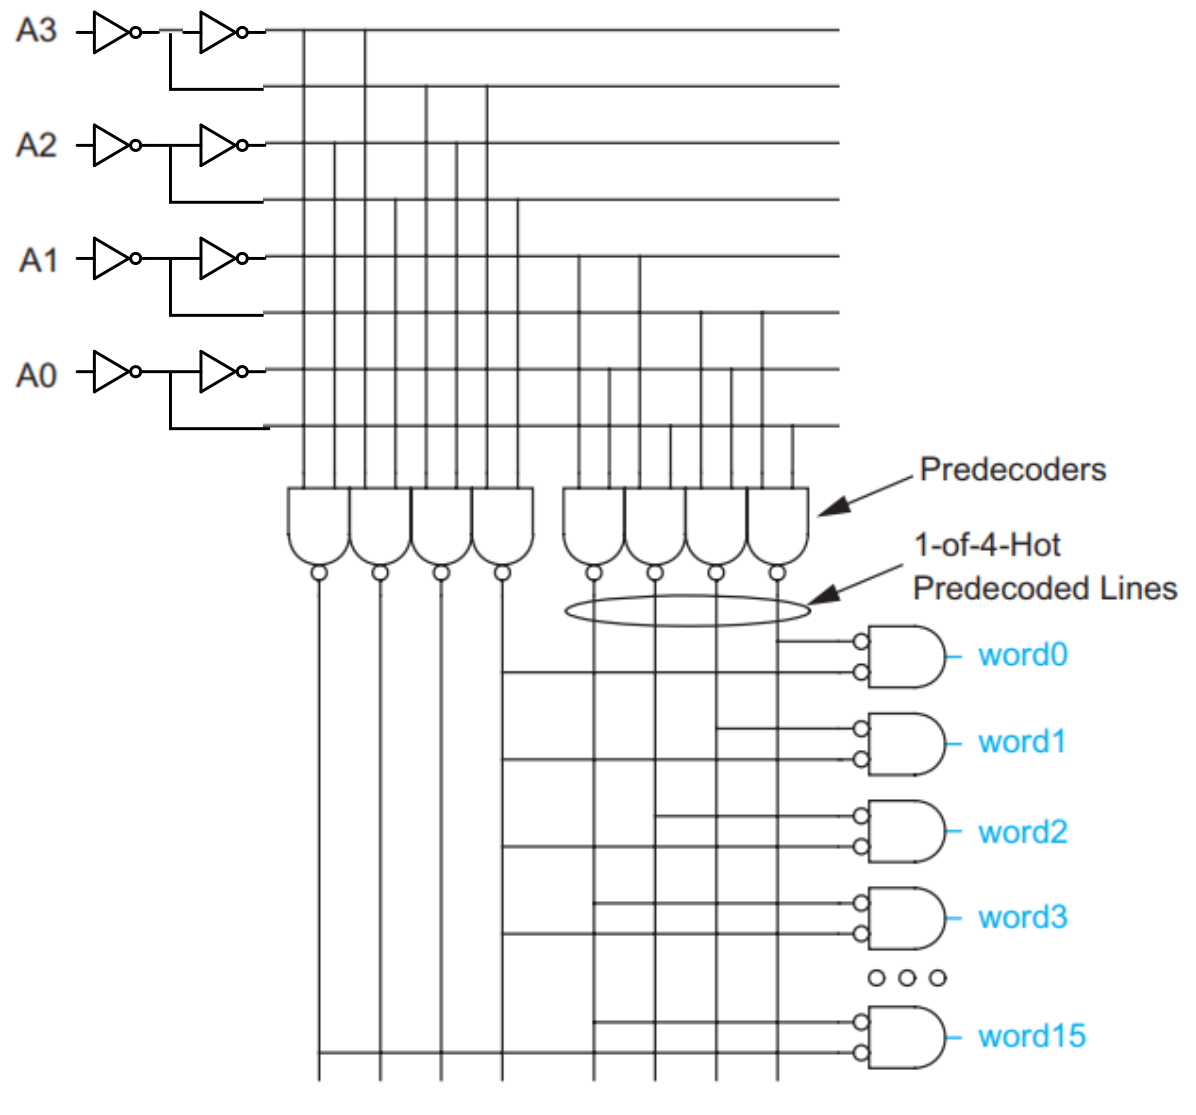
\includegraphics[width=\linewidth]{task2_ckt.png}
        \caption{4 to 16 decoder电路图}
        \label{fig:task2_ckt}
    \end{subfigure}
    \begin{subfigure}{0.48\textwidth}
        \centering
        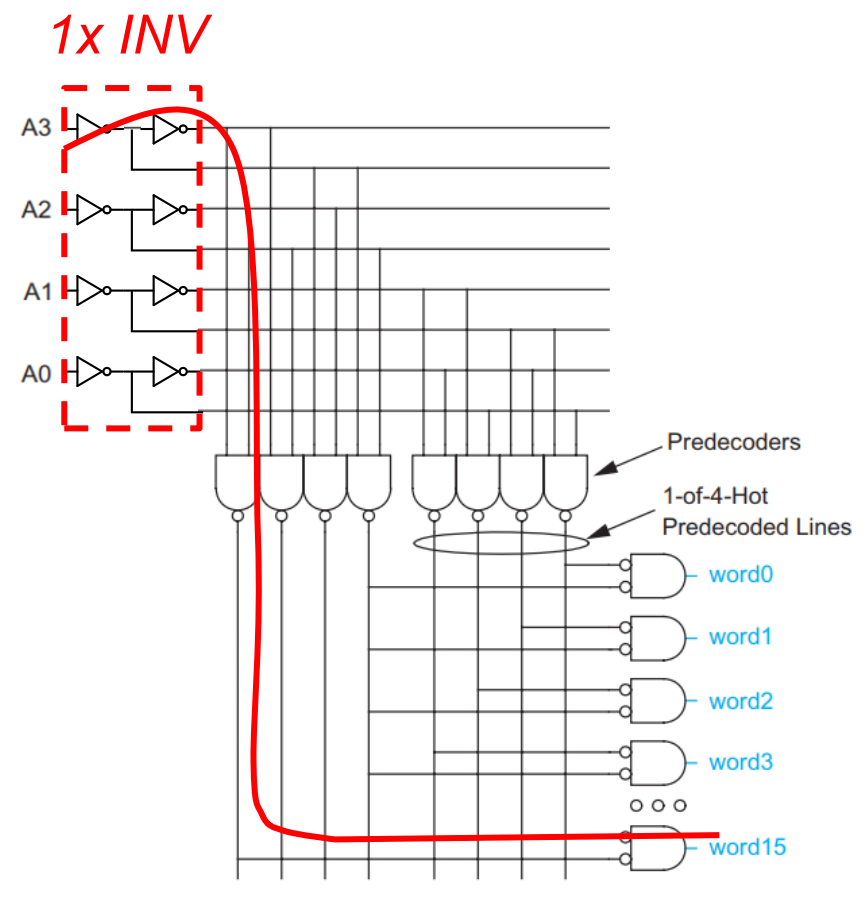
\includegraphics[width=\linewidth]{task2_ckt_withcp.png}
        \caption{4 to 16 decoder待研究的critical path}
        \label{fig:task2_ckt_withcp}
    \end{subfigure}
    \caption{4 to 16 decoder实验电路图}
    \label{fig:task2_circuit}
\end{figure}

\subsection{critical path}

由图\ref{fig:task2_circuit}不难发现，电路中的所有关键路径种类相同，即都经过了两级反相器、一级2-NAND以及以及2-NOR门，共8条。因此我们选择其中任意一条critical path讨论即可。这里选择了：

$A_3 \rightarrow \text{Xinv31} \rightarrow \text{NA}_3 \rightarrow \text{Xinv32} \rightarrow \text{PA}_3 \rightarrow \text{XNAND2\_7} \rightarrow \text{PA3\_PA2} \rightarrow \text{XNOR2\_15} \rightarrow \text{word}15 \rightarrow \text{Cload}(128\times{inv})$。

其中Xinv31、Xinv32是$A_3$经过的第一、二级反相器，\textbf{在本实验中均为最小反相器。}XNAND2\_7是$PA_3$经过的其中一个2-NAND门，XNOR2\_15是信号$PA3\_PA2$（即信号$A_{3}A_{2}$）经过的2-NOR门。

优化目标是考察从电路中第一级反相器Xinv31的输出结点（即案例中的$NA_3$）到负载电容输入结点的最小延迟，优化方法是在$\text{word}15$和负载电容间插入多级反相器作为缓冲。

\subsection{理论优化阶段}

\subsubsection{优化方法建模}

我们从已知组合逻辑门能够获取的指标（本征延迟$p$、逻辑努力$g$、尺寸$s$、等效扇出$f$、分支努力$b$）参见表\ref{tab:task2_metrics}（设Xinv32, XNAND2\_7, XNOR2\_15的参数下标分别为1, 2, 3, 4，$z_1 \sim z_m$分别代表插入的$m$级反相器）

\begin{table}[htbp]
    \centering
    \caption{Task2组合逻辑门链的逻辑门关键指标}
    \label{tab:task2_metrics}
    % 修正：原代码为6列，实际数据只有5列，改为ccccc
    \begin{tabular}{ccccc}
    \toprule
    stage & Xinv32 & XNAND2\_7 & XNOR2\_15 & $z_1 \sim z_m$ \\
    \midrule
    $p$ & $p_1 = 1$ & $p_2 = 2$ & $p_3 = 2$ & $[1,1,\cdots ,1]$ \\
    $g$ & $g_1 = 1$ & $g_2 = 3/2$ & $g_3 = 3/2$ & $[1,1,\cdots ,1]$ \\
    $s$ & $s_1 = 1$ & $s_2 = x$ & $s_3 = y$ & $[z_1, z_2, \cdots, z_m]$ \\
    $f$ & $f_1 = x$ & $f_2 = y/x$ & $f_3 = z_{1}/y$ & $[z_{2}/z_{1}, z_{3}/z_{2}, \cdots, 128/z_{m}]$ \\
    $b$ & $b_1 = 2$ & $b_2 = 4$ & $b_3 = 1$ & $[1,1,\cdots ,1]$ \\
    \bottomrule
    \end{tabular}
\end{table}

因此，通过计算，得到该链的$G,B,F,H$值/变量表示参见表\ref{tab:task2_path_metrics}。

\begin{table}[htbp]
    \centering
    \caption{Task2组合逻辑门链的路径关键指标}
    \label{tab:task2_path_metrics}
    \begin{tabularx}{\linewidth}{XXXXXX}
    \toprule
    Path logical effort($G$) & Branching effort($B$) &
    Path electrical effort($F$) & Path effort($H$) &
    Total parasitic delay($P$) & $H_{\text{min}}$ \\
    \midrule
    $\frac{9}{4}$ & 8 & 128 & $\sum_{i=1}^{m+3}{g_i f_i b_i}$ & $m+5$ & 2304  \\
    \bottomrule
    \end{tabularx}
\end{table}

因此我们有路径延迟：
$$D = (m+3) \cdot 2304^{1/(m+3)} + m + 5$$

\subsubsection{理论优化结果}

理论上通过求导和数值计算，在：
$$h_{\text{opt}} \approx 3.59, m \approx 3.05$$
时$D$有最小值：28.8039。为了更精确的分析，我们使用Task2/opt.py脚本，获得了在$m=3$附近的几个$m$值对应的$h_{\text{opt}}$以及$D_{\text{min}}$，见表\ref{tab:task2_m_opt}。
\begin{table}[htbp]
    \centering
    \caption{Task2 $m$值的理论优化选择}
    \label{tab:task2_m_opt}
    \begin{tabular}{ccc|ccc|ccc}
    \toprule
    $m$ & $h_{\text{opt}}$ & $D_{\text{min}}$ & 
    $m$ & $h_{\text{opt}}$ & $D_{\text{min}}$ & 
    $m$ & $h_{\text{opt}}$ & $D_{\text{min}}$ \\
    \midrule
    0 & 13.21 & 44.62 & 7 & 2.17 & 33.69 & 14 & 1.58 & 45.81 \\
    1 & 6.93 & 33.71 & 8 & 2.02 & 35.24 & 15 & 1.54 & 47.67 \\
    2 & 4.70 & 30.52 & 9 & 1.91 & 36.88 & 16 & 1.50 & 49.56 \\
    \textcolor{red}{3} & \textcolor{red}{3.63} & \textcolor{red}{29.81} & 10 & 1.81 & 38.58 & 17 & 1.47 & 51.45 \\
    4 & 3.02 & 30.16 & 11 & 1.74 & 40.34 & 18 & 1.45 & 53.36 \\
    5 & 2.63 & 31.06 & 12 & 1.68 & 42.13 & 19 & 1.42 & 55.28 \\
    6 & 2.36 & 32.27 & 13 & 1.62 & 43.96 & & & \\
    \bottomrule
    \end{tabular}
\end{table}

其中，等效扇出$f$，逻辑门尺寸$s$的计算方法与Task1中完全相同，\textcolor{red}{取整方法依旧采用四舍五入}，因此这里不再展示详细细节，而是\textbf{直接给出计算结果以及取整结果}。
\begin{table}[htbp]
    \centering
    \caption{Task2 通过理论计算得到的$f$, $s$最优值以及取整近似值}
    \label{tab:task2_theo_best_sf}
    \small
    \begin{tabular}{ccccc}
    \toprule
    $m$ & Xinv31 & XNAND2\_7 & XNOR2\_15 & $z_1 \sim z_m$ \\
    \midrule
    \multirow{2}{*}{$m=0$理论值} & $f_1 = 6.60$ & $f_2 = 2.20$ & $f_3 = 8.80$ & \multirow{2}{*}{[]} \\
                                 & $s_1 = 1$ & $s_2 = 6.60$ & $s_3 = 14.54$ &  \\
    $m=0$取整值 & $s_1 = 1$ & $s_2 = 7$ & $s_3 = 15$ & [] \\
    \midrule
    \multirow{2}{*}{$m=1$理论值} & $f_1 = 3.46$ & $f_2 = 1.15$ & $f_3 = 4.62$ & $f_4 = 6.93$ \\
                                 & $s_1 = 1$ & $s_2 = 3.46$ & $s_3 = 4.00$ & $s_4 = 18.48$ \\
    $m=1$取整值 & $s_1 = 1$ & $s_2 = 3$ & $s_3 = 4$ & $s_4 = 18$ \\
    \midrule
    \multirow{2}{*}{$m=2$理论值} & $f_1 = 2.35$ & $f_2 = 0.78$ & $f_3 = 3.14$ & $f_{4\sim5} = 4.70$ \\
                                 & $s_1 = 1$ & $s_2 = 2.35$ & $s_3 = 1.84$ & $[5.78, 27.21]$ \\
    $m=2$取整值 & $s_1 = 1$ & $s_2 = 2$ & $s_3 = 2$ & $[6, 27]$ \\
    \midrule
    \multirow{2}{*}{$m=3$理论值} & $f_1 = 1.82$ & $f_2 = 0.61$ & $f_3 = 2.42$ & $f_{4\sim6} = 3.63$ \\
                                 & $s_1 = 1$ & $s_2 = 1.82$ & $s_3 = 1.10$ & $[2.67, 9.69, 35.22]$ \\
    $m=3$取整值 & $s_1 = 1$ & $s_2 = 2$ & $s_3 = 1$ & $[3, 10, 35]$ \\
    \midrule
    \multirow{2}{*}{$m=4$理论值} & $f_1 = 1.51$ & $f_2 = 0.50$ & $f_3 = 2.01$ & $f_{4\sim7} = 3.02$ \\
                                 & $s_1 = 1$ & $s_2 = 1.51$ & $s_3 = 0.76$ & $[1.53, 4.64, 14.01, 42.35]$ \\
    $m=4$取整值 & $s_1 = 1$ & $s_2 = 2$ & $s_3 = 1$ & $[2, 5, 14, 42]$ \\
    \midrule
    \multirow{2}{*}{$m=5$理论值} & $f_1 = 1.32$ & $f_2 = 0.44$ & $f_3 = 1.75$ & $f_{4\sim8} = 2.63$ \\
                                 & $s_1 = 1$ & $s_2 = 1.32$ & $s_3 = 0.58$ & $[1.01, 2.67, 7.02, 18.48, 48.63]$ \\
    $m=5$取整值 & $s_1 = 1$ & $s_2 = 1$ & $s_3 = 1$ & $[1, 3, 7, 18, 49]$ \\
    \bottomrule
    \end{tabular}
\end{table}


在实际仿真过程中，我们选择了表\ref{tab:task2_m_opt}中较为不错的$D_{\text{min}}$结果对应的$m$，进行进一步查看，判断在$m=3$、最优尺寸参数组合下，电路critical path是否真的具有最低延迟$t_{\text{p}}$。

\subsection{HSPICE仿真阶段}

\subsubsection{插入反相器级数的进一步确定}

虽然理论上在$m = 3$时达到最优延迟，但实际情况可能有出入。因此对$m = 0$到$m = 5$的情况进行了仿真，每种情况采用对应的最优尺寸参数。仿真结果如表\ref{tab:task2_m}所示。

\begin{table}[htbp]
\centering
\caption{不同反相器级数m的延迟结果}
\label{tab:task2_m}
\begin{tabular}{cccc}
\toprule
$m$ & $t_{pLH}$(ps) & $t_{pHL}$(ps) & $t_p$(ps) \\
\midrule
0 & 63.48 & 43.60 & 53.54 \\
1 & 35.59 & 46.13 & 40.86 \\
\textcolor{red}{2} & \textcolor{red}{42.41} & \textcolor{red}{33.22} & \textcolor{red}{37.81} \\
\textcolor{blue}{3} & \textcolor{blue}{34.77} & \textcolor{blue}{42.07} & \textcolor{blue}{38.42} \\
4 & 42.19 & 35.52 & 38.86 \\
5 & 36.87 & 42.43 & 39.65 \\
\bottomrule
\end{tabular}
\end{table}

可以发现，实际上在$m = 2$时有最优延迟（$t_p = 37.81$ps），与理论预测的$m = 3$有所不同。但是两者非常接近，延迟差距也很小。这样暗示着我们，\textbf{理论分析的结果作用不是直接帮助我们确定最优解，而是给我们提供了一个最优解可能存在的局部范围，我们需要借助仿真工具进一步在这个局部范围里进行微调，从而得到更精确的最优解。}

\subsubsection{尺寸参数的精细扫描}

根据以上结果，我们不仅在$m = 2$时扫描参数，还在临近的$m = 1$和$m = 3$时同时扫描，尽可能扩大范围得到最优延迟。三种情况的参数扫描范围如下：

对于$m = 1$：XNAND2\_size扫描范围为[2, 3, 4]，XNOR2\_size扫描范围为[3, 4, 5]，buffer\_0\_size扫描范围为[14, 16, 18, 20, 22]。

对于$m = 2$：XNAND2\_size扫描范围为[1, 2, 3]，XNOR2\_size扫描范围为[1, 2, 3]，buffer\_0\_size扫描范围为[4, 5, 6, 7, 8]，buffer\_1\_size扫描范围为[21, 24, 27, 30, 33]。

对于$m = 3$：XNAND2\_size扫描范围为[1, 2, 3]，XNOR2\_size扫描范围为[1, 2]，buffer\_0\_size扫描范围为[2, 3, 4]，buffer\_1\_size扫描范围为[8, 11, 14]，buffer\_2\_size扫描范围为[28, 33, 38]。

\subsubsection{仿真结果与分析}

三种情况的最优尺寸参数及对应延迟如下（或者参见表\ref{tab:task2_parc_best_tp}）：

$m = 1$时：XNAND2\_size = 3，XNOR2\_size = 5，z1\_size = 18，得到$t_{pLH} = 35.61$ps，$t_{pHL} = 45.95$ps，$t_p = 40.78$ps。

$m = 2$时：XNAND2\_size = 2，XNOR2\_size = 2，z1\_size = 6，z2\_size = 24，得到$t_{pLH} = 42.34$ps，$t_{pHL} = 33.04$ps，$t_p = 37.69$ps。

$m = 3$时：XNAND2\_size = 1，XNOR2\_size = 1，z1\_size = 2，z2\_size = 8，z3\_size = 28，得到$t_{pLH} = 34.22$ps，$t_{pHL} = 40.70$ps，$t_p = 37.46$ps。

\begin{table}[htbp]
\centering
\caption{Task2 各$m$对应的最优延迟以及尺寸参数组合}
\label{tab:task2_parc_best_tp}
\begin{tabular}{ccccccc}
\toprule
$m$ & XNAND2\_7 & XNOR2\_15 & $z_1 \sim z_m$ &$t_{pLH}$(ps) & $t_{pHL}$(ps) & $t_p$(ps) \\
\midrule
1 & 3 & 5 & $[18]$ & 35.61 & 45.95 & 40.78 \\
2 & 2 & 2 & $[6, 24]$ & 42.34 & 33.04 & 37.69 \\
3 & 1 & 1 & $[2, 8, 28]$ & 34.22 & 40.70 & 37.46 \\
\bottomrule
\end{tabular}
\end{table}

综合以上结果，在$m = 3$时获得了最优延迟$t_p = 37.46$ps。

在最优解情况下，\textbf{电路详细尺寸参数为：}

\textbf{1.} 关键路径为：

$A_3 \rightarrow \text{Xinv31} \rightarrow \text{NA}_3 \rightarrow \text{Xinv32} \rightarrow \text{PA}_3 \rightarrow \text{XNAND2\_7} \rightarrow \text{PA3\_PA2} \rightarrow \text{XNOR2\_15} \rightarrow \text{word}15 \rightarrow z_1 \rightarrow z_2 \rightarrow z_3 \rightarrow \text{Cload}(128\times{inv})$。

\textbf{2.} 各门的逻辑努力、尺寸等参数如表\ref{tab:task2_best_gate_params}所示。

\begin{table}[htbp]
\centering
\caption{Task2 critical path各逻辑门最优尺寸参数组合}
\label{tab:task2_best_gate_params}
\begin{tabular}{ccccc}
\toprule
逻辑门 & 尺寸$s$ & 逻辑努力$g$ & 分支努力$b$ & 等效扇出$f$ \\
\midrule
Xinv32    & 1 & 1 & 2 & 1 \\
XNAND2\_7 & 1 & 3/2 & 4 & 1 \\
XNOR2\_15 & 1 & 3/2 & 1 & 2 \\
$z_1$     & 2 & 1 & 1 & 4 \\
$z_2$     & 8 & 1 & 1 & 3.5 \\
$z_3$     & 28 & 1 & 1 & 4.57 \\
\bottomrule
\end{tabular}
\end{table}

\textbf{3.} critical path路径参数见\ref{tab:task2_best_path_params}
$G = 1 \times 3/2 \times 3/2 \times 1 \times 1 \times 1 = 9/4 $，$B = 8 $，
$B = 8$，
$F = 1\times 1\times 2 \times 4 \times 3.5 \times 4.57 = 127.96 \approx 128$，
$H = GBF = 9/4 \times 8 \times 127.96 \approx 2304$。

\begin{table}[htbp]
    \centering
    \caption{Task2 critical path最优路径参数}
    \label{tab:task2_best_path_params}
    \begin{tabularx}{\linewidth}{XXXXXX}
    \toprule
    Path logical effort($G$) & Branching effort($B$) &
    Path electrical effort($F$) & Path effort($H$) &
    Total parasitic delay($P$) & $D_{\text{min}}$ \\
    \midrule
    $\frac{9}{4}$ & 8 & 128 & 2304 & 8 &  29.80 \\
    \bottomrule
    \end{tabularx}
\end{table}

%================================================================================
% Task 3: Use Logical Effort to Optimize 5×32 Decoder
%================================================================================
\newpage
\section{Task 3: Use Logical Effort to Optimize 5$\times$32 Decoder}

\subsection{实验电路}

本任务利用互补逻辑门搭建一个完整的5 to 32解码器。电路结构包含：第一层5个反相器，输入$A_4$, $A_3$, $A_2$, $A_1$, $A_0$，输出$NA_4$, $NA_3$, $NA_2$, $NA_1$, $NA_0$；第二层5个反相器，输出$PA_4$, $PA_3$, $PA_2$, $PA_1$, $PA_0$；第三层包含1个反相器（生成$NPA_0$）和8个NAND2门；最后一层是32个NOR3门，输出$word_0$到$word_{31}$。负载电容等效于256倍最小反相器尺寸的反相器。

与Task 2不同的是，本任务存在两条不同的关键路径：

关键路径1（H1\_pro）：$A_0 \rightarrow \text{Xinv01} \rightarrow \text{NA}_0 \rightarrow \text{Xinv02} \rightarrow \text{PA}_0 \rightarrow \text{XinvPA0} \rightarrow \text{NPA}_0 \rightarrow \text{XNOR3\_1} \rightarrow \text{word}_1$

关键路径2（H2）：$A_1 \rightarrow \text{Xinv11} \rightarrow \text{NA}_1 \rightarrow \text{Xinv12} \rightarrow \text{PA}_1 \rightarrow \text{XNAND2\_1} \rightarrow \text{NA2\_PA1} \rightarrow \text{XNOR3\_2} \rightarrow \text{word}_2$

这两条关键路径独立考虑，给出对应两组最优参数。

\subsection{理论优化阶段}

\subsubsection{优化方法建模}
（待完善）

\subsubsection{理论优化结果}

通过理论分析和数值计算，得到以下结果（其中$N = m + 3$表示关键路径上的总级数）：

对于关键路径H1\_pro，当$m = 4$（$N = 7$）时，$D = 35.36$，$h_{\text{opt}} = 3.62$。

对于关键路径H2，当$m = 4$（$N = 7$）时，$D = 36.87$，$h_{\text{opt}} = 3.84$。

\subsection{HSPICE仿真阶段}

\subsubsection{插入反相器级数的进一步确定}

虽然理论上H1\_pro和H2都在$m = 4$时达到最优延迟，但实际情况可能有出入。因此分别对不同$m$值进行了仿真验证。

对于H1\_pro，$m$从1到8进行扫描；对于H2，$m$从2到8进行扫描。仿真结果如表\ref{tab:task3_m_H1pro}和表\ref{tab:task3_m_H2}所示。

\begin{table}[htbp]
\centering
\caption{H1\_pro：不同反相器级数m的延迟结果}
\label{tab:task3_m_H1pro}
\begin{tabular}{cccc}
\toprule
$m$ & $t_{pLH}$(ps) & $t_{pHL}$(ps) & $t_p$(ps) \\
\midrule
1 & 151.8 & 167.9 & 159.9 \\
2 & 90.62 & 78.44 & 84.53 \\
\textcolor{red}{3} & \textcolor{red}{60.15} & \textcolor{red}{68.99} & \textcolor{red}{64.57} \\
4 & 67.98 & 62.36 & 65.17 \\
5 & 63.25 & 68.02 & 65.63 \\
6 & 69.23 & 64.15 & 66.69 \\
7 & 69.19 & 73.39 & 71.29 \\
8 & 75.07 & 70.60 & 72.84 \\
\bottomrule
\end{tabular}
\end{table}

\begin{table}[htbp]
\centering
\caption{H2：不同反相器级数m的延迟结果}
\label{tab:task3_m_H2}
\begin{tabular}{cccc}
\toprule
$m$ & $t_{pLH}$(ps) & $t_{pHL}$(ps) & $t_p$(ps) \\
\midrule
2 & 62.43 & 47.15 & 54.79 \\
\textcolor{red}{3} & \textcolor{red}{44.16} & \textcolor{red}{52.57} & \textcolor{red}{48.37} \\
4 & 52.36 & 44.58 & 48.47 \\
5 & 45.37 & 51.95 & 48.66 \\
6 & 56.06 & 47.06 & 51.56 \\
7 & 48.75 & 56.98 & 52.86 \\
8 & 59.41 & 51.00 & 55.20 \\
\bottomrule
\end{tabular}
\end{table}

由表\ref{tab:task3_m_H1pro}和表\ref{tab:task3_m_H2}可以发现，H1\_pro在$m = 3$时有最优延迟（$t_p = 64.57$ps），H2在$m = 3$时有最优延迟（$t_p = 48.37$ps），两者均与理论预测的$m = 4$有所不同，但两者非常接近。这再次印证了\textbf{理论分析的结果作用不是直接帮助我们确定最优解，而是给我们提供了一个最优解可能存在的局部范围。}

\subsubsection{尺寸参数的精细扫描}

根据以上结果，在H1\_pro和H2均选择$m = 3$进行精细参数扫描。参数扫描范围如下：

对于H1\_pro（$m = 3$）：XinvPA0\_size扫描范围为[3, 4, 5]，XNAND2\_size扫描范围为[3, 4, 5]，XNOR3\_size扫描范围为[1, 2]，buffer\_0\_size扫描范围为[2, 3, 4]，buffer\_1\_size扫描范围为[11, 13, 15]，buffer\_2\_size扫描范围为[48, 51, 54, 57, 60, 63, 66]。

对于H2（$m = 3$）：XinvPA0\_size扫描范围为[1, 2, 3]，XNAND2\_size扫描范围为[1, 2, 3]，XNOR3\_size扫描范围为[1, 2]，buffer\_0\_size扫描范围为[1, 2, 3]，buffer\_1\_size扫描范围为[6, 8, 10]，buffer\_2\_size扫描范围为[31, 34, 37, 40, 43, 46, 49]。

\subsubsection{仿真结果与分析}

两种关键路径的最优尺寸参数及对应延迟如下（参见表\ref{tab:task3_parc_best_tp}）：

H1\_pro（$m = 3$）时：XinvPA0\_size = 5，XNAND2\_size = 3，XNOR3\_size = 1，buffer\_0\_size = 3，buffer\_1\_size = 11，buffer\_2\_size = 48，得到$t_{pLH} = 59.77$ps，$t_{pHL} = 68.62$ps，$t_p = 64.19$ps。

H2（$m = 3$）时：XinvPA0\_size = 1，XNAND2\_size = 2，XNOR3\_size = 1，buffer\_0\_size = 3，buffer\_1\_size = 10，buffer\_2\_size = 43，得到$t_{pLH} = 43.06$ps，$t_{pHL} = 53.52$ps，$t_p = 48.29$ps。

\begin{table}[htbp]
\centering
\caption{Task3 各关键路径对应的最优延迟以及尺寸参数组合}
\label{tab:task3_parc_best_tp}
\begin{tabular}{cccccccc}
\toprule
路径 & XinvPA0 & XNAND2 & XNOR3 & $z_1, z_2, z_3$ & $t_{pLH}$(ps) & $t_{pHL}$(ps) & $t_p$(ps) \\
\midrule
H1\_pro & 5 & 3 & 1 & $[3, 11, 48]$ & 59.77 & 68.62 & 64.19 \\
H2 & 1 & 2 & 1 & $[3, 10, 43]$ & 43.06 & 53.52 & 48.29 \\
\bottomrule
\end{tabular}
\end{table}

综合以上结果，在两条关键路径中，H2的延迟更小，为$t_p = 48.29$ps。（待完善）

\end{document}
